\section{How it Works}

	\subsection{Grayscale Square Images}

	We will first try our hands upon a grayscale images. Grayscale images are images in which every pixel has a single brightness value. So it is easier to work with.
	
	After Importing all the classes and functions\footnote{All the relevant functions and classes have been kept in: \href{https://github.com/PeithonKing/comp_phys_P346/blob/main/library/DIY.py}{the Library File}} from the library file, we can make an instance of the \href{https://github.com/PeithonKing/comp_phys_P346/blob/main/library/DIY.py#L43-L69}{\textbf{GrayscaleImageSVD}} class. This class takes the location of the image as an input. When the instance is constructed, it loads the image to it's memory as a numpy array. Then it callculates the U, S and V matrices using the \href{https://numpy.org/doc/stable/reference/generated/numpy.linalg.svd.html}{\textbf{numpy.linalg.svd()}} function from the \href{https://numpy.org/}{\textbf{NumPy}} library.
	\vspace{2mm}

	\begin{center}
		\noindent\fbox{
			\parbox{0.95\columnwidth}{
			\textbf{Using \href{https://numpy.org/doc/stable/reference/generated/numpy.linalg.svd.html}{numpy.linalg.svd()} function:} We can use the \href{https://numpy.org/doc/stable/reference/generated/numpy.linalg.svd.html}{$numpy.linalg.svd()$} function to compute the SVD of a matrix. The function returns the $3$ matrices: $U$, $S$ and $V$. In the $S$ matrix, we get the singular values in descending order. The function returns the matrix $S$ not in the form of a diagonal matrix but as a vector of singular values. So, we will have to convert it into a diagonal matrix (by \href{https://numpy.org/doc/stable/reference/generated/numpy.diag.html}{$numpy.diag()$} function) before we can use it to reconstruct the matrix $A$.
			}
		}
	\end{center}

	\begin{lstlisting}[language=Python]
from library.DIY import GrayscaleImageSVD
pic = "monkey"
img = GrayscaleImageSVD(f"static/{pic}.jpg")
img.display("Original Square Grayscale Image")
	\end{lstlisting}
	
	\begin{figure}[H]
		\centering
		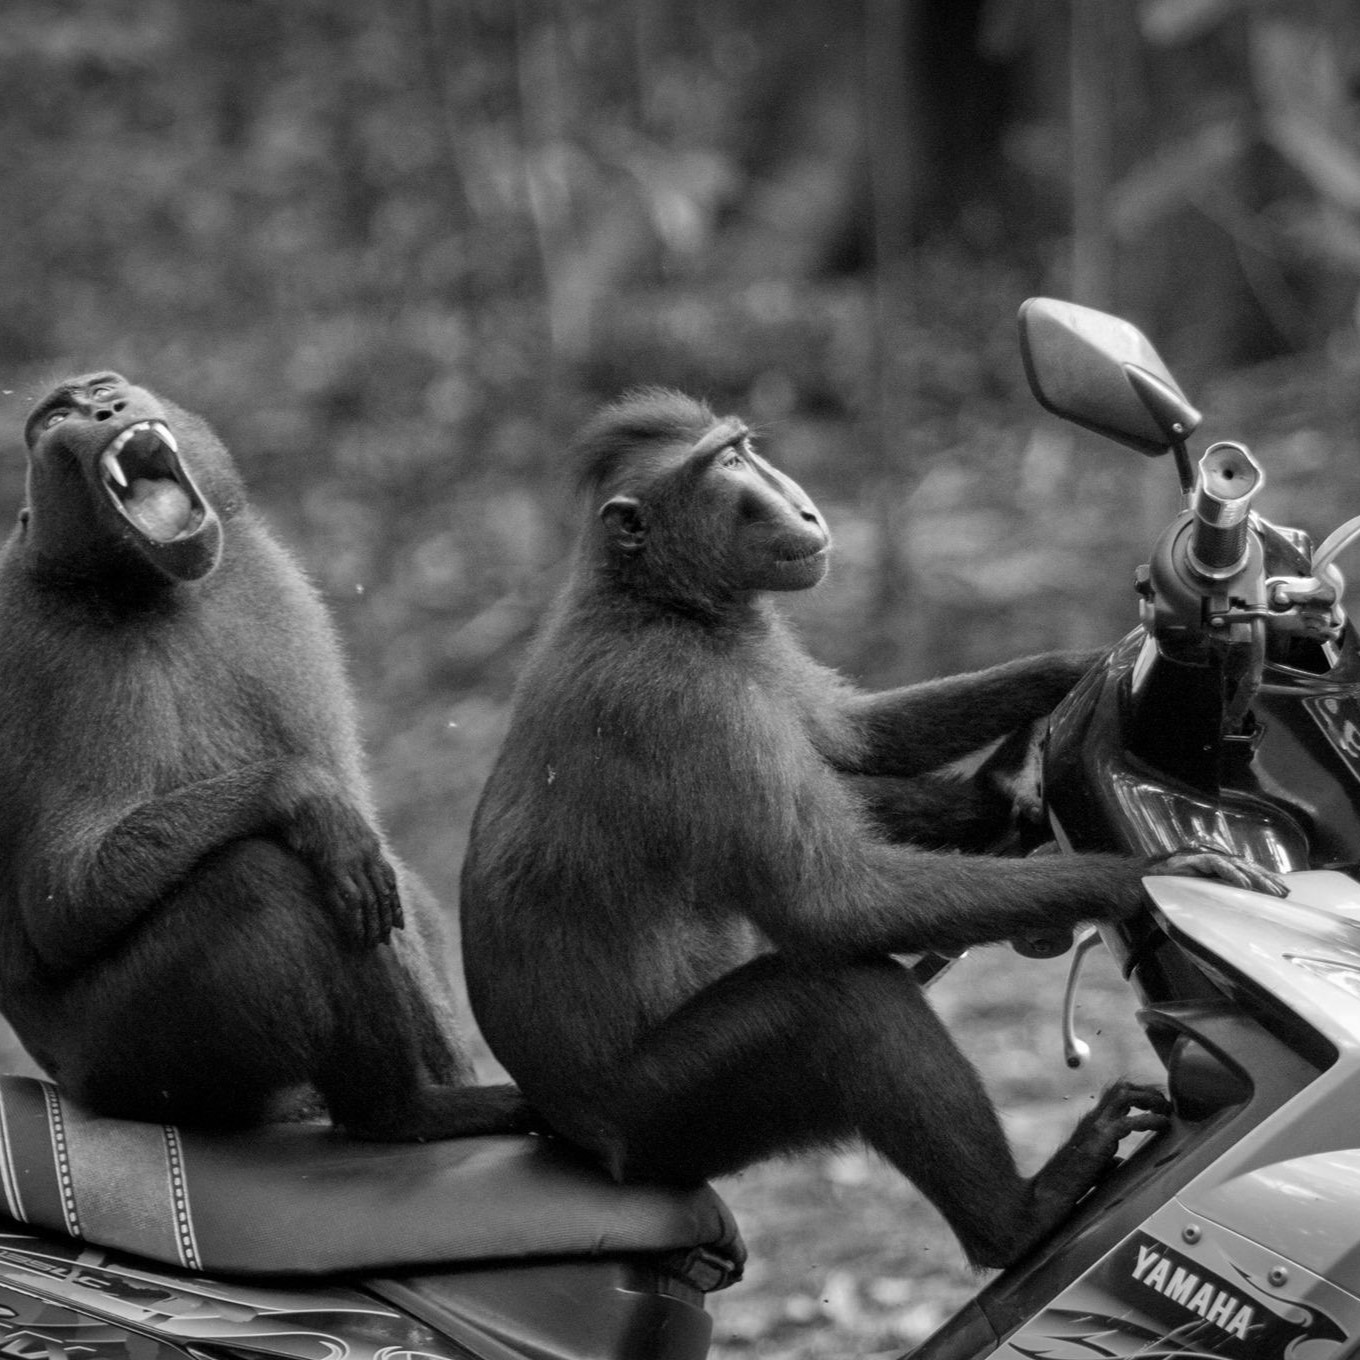
\includegraphics[width=0.35\textwidth]{../static/monkey/monkey.jpg}
		\caption{Original Square Grayscale Image}
		\label{fig:g_monkey_orig}
	\end{figure}

	Next, we can call the \href{https://github.com/PeithonKing/comp_phys_P346/blob/main/library/DIY.py#L55-L59}{\textbf{GrayscaleImageSVD.reduce()}} method to get the reduced image. This function takes the number of singular values to be used as an input. It then uses the first $n$ singular values to reconstruct the image. The function returns the reconstructed image as a numpy array. We can then use the \textbf{show\_image()} function to display the image. Note that, the returned array is not smaller in size than the original image; it is a full sized image. But this array can be constructed using arrays of much smaller sizes.

	Although we have writen our own SVD function \href{google.com}{(demonstration \textbf{here})}, we won't be actually using that for this project.

	\begin{center}
		\noindent\fbox{
			\parbox{0.95\columnwidth}{
				\textbf{Why are we using the SVD function from numpy and not using the SVD function which is our own?}
				This is because the SVD function from numpy is written in C and is highly optimized. So, it is much faster than our own implementation. Moreover finding SVD of a matrix involves finding eigenvalues and eigenvectors of the matrix. We know that the algorithms studied in this class become inefficient if we are working with a large matrix. The later values have a lot of error in them. So, writing the SVD function is itself a huge problem to be solved. On the other hand, finding SVD of a matrix is a very well studied problem in literature and there are many efficient algorithms to find it. So, we can use the SVD function from numpy without reinventing the wheel.
			}
		}
	\end{center}

